\section{Calcul d'erreurs}
\label{sec:erreurs}

Les erreurs sur les mesures sont données dans le \autoref{tab:erreurs}.

\begin{table}[h]
    \centering
    \begin{tabulary}{\textwidth}{C C}
        \toprule
        Variable & Erreur \\
        \midrule
        \(L_\textrm{échantillon}\) [\si{\centi\meter}] & 0.1 \\
        \(\delta_\textrm{laser}\) [\si{\centi\meter}] & 0.2 \\
        \(m_\textrm{sus}\) [\si{\gram}] & 5 \\
        \(a\) [\si{\centi\metre}] & 0.3 \\
        \(D\) [\si{\centi\metre}] & 0.005 \\
        \(d\) [\si{\centi\meter}] & 0.001 \\
        \(\ell\) [\si{\centi\meter}] & 0.005 \\
        \bottomrule
    \end{tabulary}
    \caption{Erreurs estimées sur les mesures}
    \label{tab:erreurs}
\end{table}

\paragraph*{Regression linéaire}
Les erreurs sur les régressions linéaires \(y = ax + b\) sur les mesures \((x_i, y_i) ; i = \{1, \dots, n\}\) sont donnés par \cite{erreursmesure}:

\begin{equation}
    \label{eq:erreur:fit}
    \begin{aligned}
        (\Delta a)^2 &= \frac{\sum_{i=1}^{n}(y_i - (a x_i + b))^2}{(n-2) \sum_{i=1}^{n}(x_i - \bar{x})^2}\\
        \Delta b &= \bar{x} \Delta a + a \Delta \bar{x}
    \end{aligned}
\end{equation}

En pratique, ces valeurs sont calculées par la bibliothèque python \texttt{numpy}.


\paragraph*{Formules d'erreurs}

Erreur sur l'angle de déformation:
\begin{equation}
    \Delta \theta = \absfrac{D}{\delta^2 + D^2} \Delta \delta + \absfrac{\delta}{\delta^2 + D^2} \Delta D
\end{equation}

Toutes ces erreurs sont calculées en pratique par la bibliothèque \texttt{uncertainties}.

\section{Figures supplémentaires}
\label{sec:figsup}

\begin{figure}[h]
    \centering
    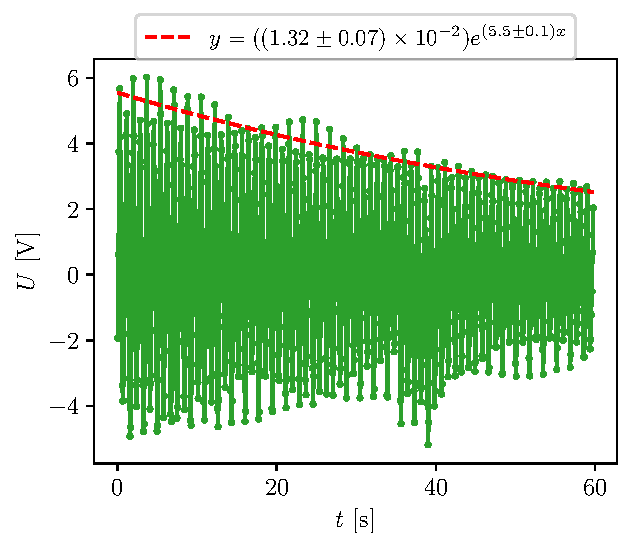
\includegraphics[width=0.6\linewidth]{figures/magnesium1.pdf}
    \caption{Amplitude des oscillation d'un échantillon de magnésium pour la méthode dynamique}
    \label{fig:dynamique_magnesium_feur}
\end{figure}
